\documentclass[tikz,convert=false]{standalone}
\usetikzlibrary{mindmap,trees,graphs,calc}
\tikzset{
  set angles for level/.style={level #1/.append style={sibling angle=360/\the\tikznumberofchildren}},
  level/.append style={set angles for level=#1}% solution 1
}
\begin{document}
\tikzset{
  set angles for level/.style={level #1/.append style={sibling angle=360/\the\tikznumberofchildren}},
  level/.append style={set angles for level=#1}% solution 1
}
\tikzset{level 1 concept/.append style={font=\sf, sibling angle=90,level distance = 25mm}}
\tikzset{level 2 concept/.append style={font=\sf, sibling angle=45,level distance = 15mm}}
\tikzset{level 3 concept/.append style={font=\sf, sibling angle=45,level distance = 15mm}}
\tikzset{every node/.append style={scale=0.6}}
% \tikzset{every node/.append style={scale=0.6}}
 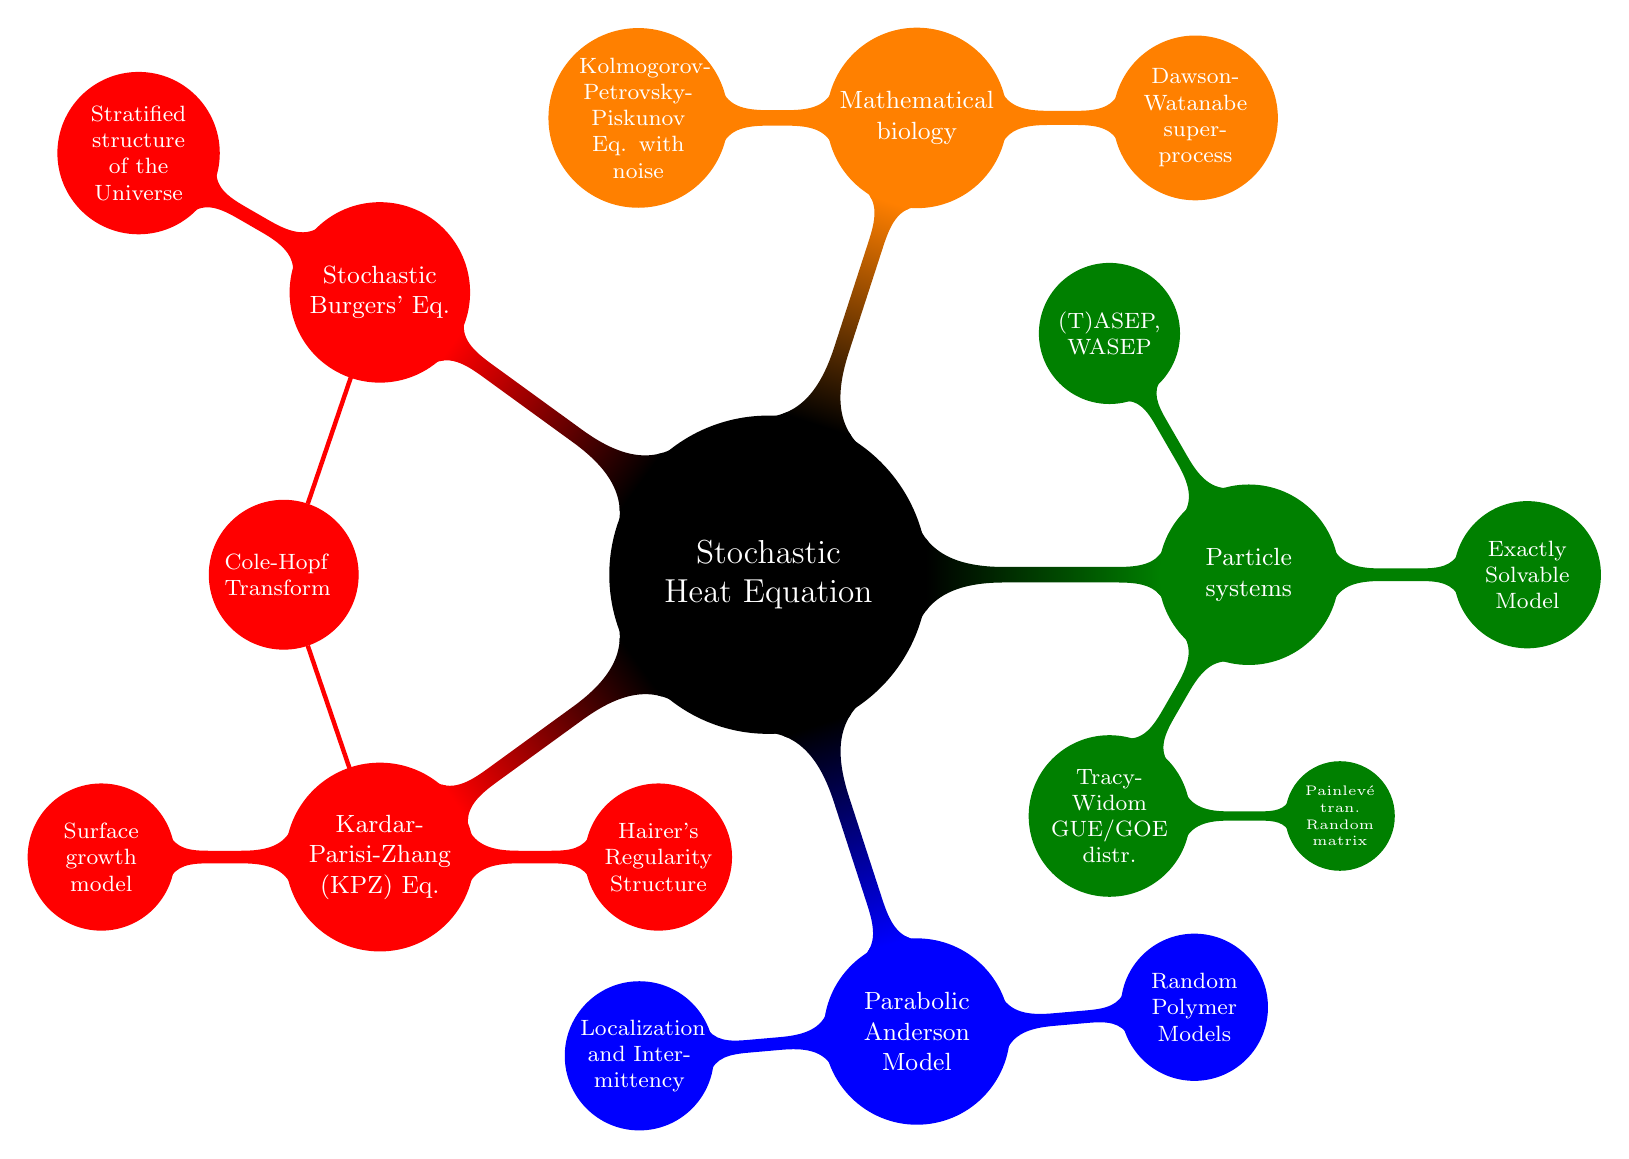
\begin{tikzpicture}[scale=1.22] 
  \path[mindmap,concept color=black,text=white]
    node[concept] {Stochastic Heat Equation}
    [clockwise from=0]
    child[concept color=green!50!black] {
      node[concept] {Particle systems} [clockwise from=120,sibling angle=30]
      child { node[concept] {(T)ASEP, \\ WASEP} 
       }
       child { node[concept] {Exactly Solvable Model}}
       child { node[concept] {Tracy-Widom GUE/GOE distr. }[clockwise from=0,sibling angle=30]
       child { node[concept] {Painlev\'e tran.\\
       Random matrix}}
       }
%       child { node[concept] {WASEP} }
%       child { node[concept] {software engineer\-ing} }
    }  
    child[concept color=blue] {
      node[concept] {Parabolic Anderson Model}
      [clockwise from=5]
      child { node[concept] {Random Polymer Models} }
      child { node[concept] {Localization and Intermittency} }
    }
    child[concept color=red] { node[concept] (KPZ) {Kardar-Parisi-Zhang (KPZ) Eq.}
    [clockwise from=180,sibling angle=-90]
    child { node[concept] {Surface growth model} }
    child { node[concept] {Hairer's Regularity Structure} }
    }
        child[concept color=red] { node[concept] (Burgers) {Stochastic Burgers' Eq.}
    [clockwise from=150]
    child { node[concept] {Stratified structure of the Universe} }}
    child[concept color=orange] { node[concept] {Mathematical biology}[clockwise from=0]
    child { node[concept] { Dawson-Watanabe superprocess}} 
    child { node[concept] {Kolmogorov-Petrovsky-Piskunov Eq. with noise}} 
    };
  \node[circle,extra concept,text=white,concept color=red] (additional) at ($(Burgers)!0.5!(KPZ)+(-1,0)$) {Cole-Hopf \\Transform}; 
   \draw[ultra thick,red] (additional) -- (KPZ);
   \draw[ultra thick,red] (additional) -- (Burgers);
\end{tikzpicture}
\end{document}
